\section{Компенсирующий регулятор по состоянию}
\subsection{Анализ системы}
\label{sec:task1}
Рассмотрим систему 
\begin{equation}
    \dot x=Ax+Bu+B_fw_f,\quad x(0)=\begin{bmatrix}
        0&0&0
    \end{bmatrix}^T,
    \label{eq:sys1}
\end{equation}
генератор внешнего возмущения
\begin{equation*}
    \dot w_f=\Gamma w_f,\quad w_f(0)=\begin{bmatrix}
        1&1&1&1
    \end{bmatrix}^T
\end{equation*}
и виртуальный выход вида
\begin{equation*}
    z=C_Zx,
\end{equation*}
где
\begin{equation*}
    A=\begin{bmatrix}
        3&5&4\\
        -2&-4&-5\\
        2&2&3
    \end{bmatrix},\quad
    B=\begin{bmatrix}
        2\\-1\\1
    \end{bmatrix},\quad
    B_f=\begin{bmatrix}
        -2&0&0&2\\
        -2&0&0&0\\
        0&0&0&0
    \end{bmatrix},\quad
\end{equation*}
\begin{equation*}
    \Gamma=\begin{bmatrix}
        35&56&22&-42\\
        -11&-17&-7&12\\
        -6&-10&-5&10\\
        11&18&6&-13
    \end{bmatrix},\quad
    C_Z=\begin{bmatrix}
        2&3&3
    \end{bmatrix}.
\end{equation*}
Собственные числа матрицы $\Gamma$
\begin{equation*}
    \sigma(\Gamma)=\{\pm3i,\ \pm i\},
\end{equation*}
внешнее возмущение имеет вид суммы гармоник:
\begin{equation*}
    w_i(t)=a_i\cos(t)+b_i\sin(t) + c_i\cos(3t)+d_i\sin(3t).
\end{equation*}
Построим схему моделирования системы \eqref{eq:sys1},
замкнутой компенсирующим регулятором
\begin{equation}
    u=K_1x+K_2w_f,
    \label{eq:reg1}
\end{equation}
обеспечивающим выполнение целевого условия
\begin{equation*}
    \lim_{t\rightarrow\infty}z(t)=0.
\end{equation*}
Схему можно увидеть на \autoref{fig:sys1}.
Проверим стабилизируема ли система (пара ($A$, $B$)).
\begin{equation*}
    \sigma(A)=\{2\pm i,\ -i\},
\end{equation*}
\begin{equation*}
    H_1=\begin{bmatrix}
        -1 + i & -5 & -4 & 2 \\
        2 & 6 + i & 5 & -1 \\
        -2 & -2 & -1 + i & 1
    \end{bmatrix},\quad \text{rank}(H_1)=3,
\end{equation*}
\begin{equation*}
    H_2=\begin{bmatrix}
        -1 - i & -5 & -4 & 2 \\
        2 & 6 - i & 5 & -1 \\
        -2 & -2 & -1 - i & 1
    \end{bmatrix},\quad \text{rank}(H_2)=3,
\end{equation*}
\begin{equation*}
    H_3=\begin{bmatrix}
        -5 & -5 & -4 & 2 \\
        2 & 2 & 5 & -1 \\
        -2 & -2 & -5 & 1
    \end{bmatrix},\quad \text{rank}(H_3)=2.
\end{equation*}
Пара ($A$, $B$) не является полностью управляемой, но
стабилизируема, этого достаточно для синтеза регулятора.

\begin{figure}[H]
    \centering
    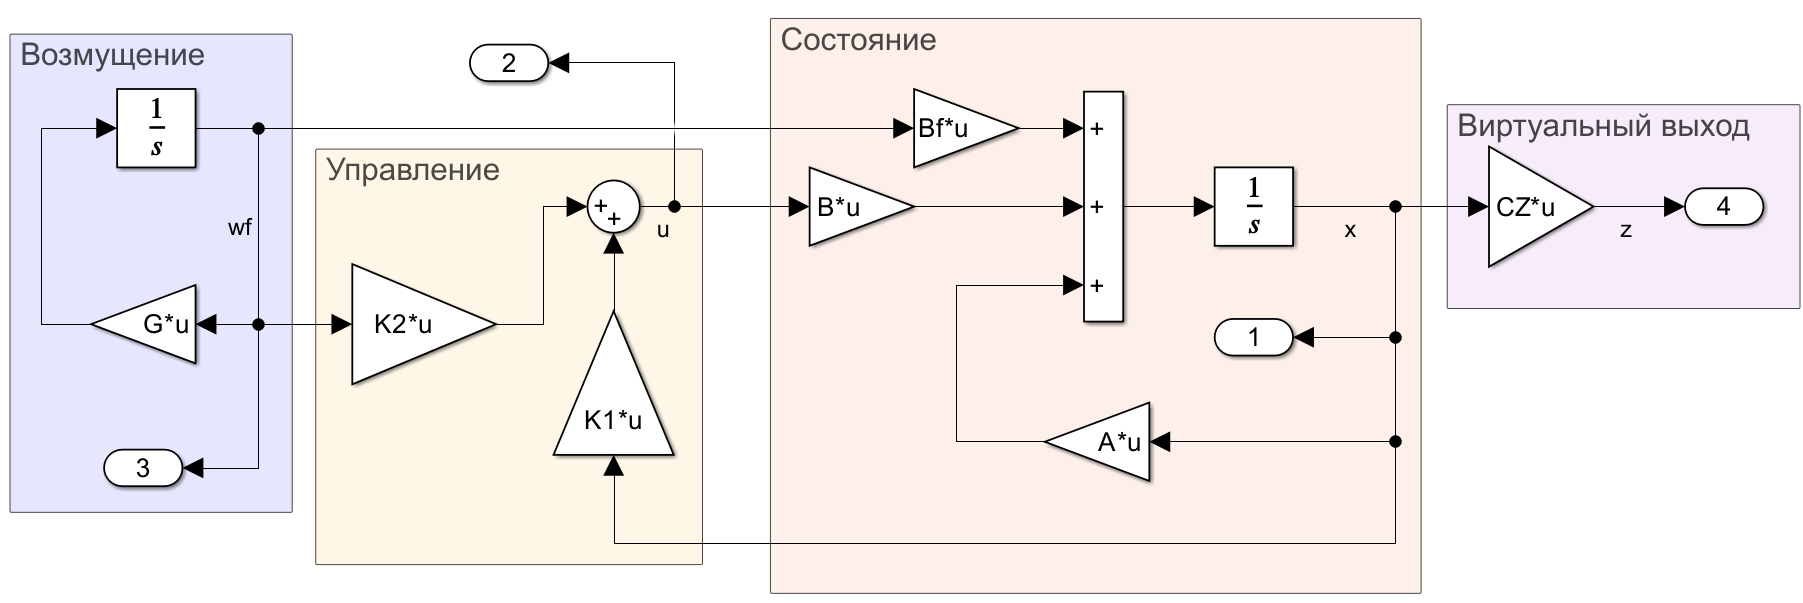
\includegraphics[width=\linewidth]{figs/task1_slx.png}
    \caption{Схема моделирования системы \eqref{eq:sys1},
    замкнутой компенсирующим регулятором \eqref{eq:reg1}}
    \label{fig:sys1}
\end{figure}

\subsection{Синтез ``feedback''-компоненты}
\label{sec:feedback1}
Синтезируем «feedback»-компоненту $K_1$ компенсирующего регулятора \eqref{eq:reg1}
с помощью уравнения Сильвестра:
\begin{equation}
    \label{eq:silv}
    AP-P\Gamma_R=BY,\quad K=-YP^{-1}.
\end{equation}
Но сначала нужно усечть систему. Найдем жордановые формы матриц:
\begin{equation*}
    A_J=\begin{bmatrix}
        -2&     0&     0\\
        0&     2&    -1\\
        0&     1&     2   
    \end{bmatrix},\quad
    B_J=\begin{bmatrix}
        0\\
        0.7071\\
       -2.1213
    \end{bmatrix},\quad
    P_J = \begin{bmatrix}
        -1&    0.7071&   -0.7071\\
        1&   -1.4142&         0\\
             0    &1.4142&         0
    \end{bmatrix},
\end{equation*}
где $P_J$ - матрица перехода. Усечем до следущих матриц:
\begin{equation*}
    A_j=\begin{bmatrix}
        2&    -1\\
        1&     2   
    \end{bmatrix},\quad
    B_j=\begin{bmatrix}
        0.7071\\
       -2.1213
    \end{bmatrix}.
\end{equation*}
возьмем следующие матрицы $\Gamma_R$ и $Y$, чтобы итоговый спект был устойчив и
пара ($\Gamma_R$, $Y$) наблюдаема
\begin{equation*}
    \Gamma_R=\begin{bmatrix}
        -10 & 1\\0&-10
    \end{bmatrix},\quad
    Y=\begin{bmatrix}
        1 & 0
    \end{bmatrix}.
\end{equation*}
Используя CVX получим следующую матрицу регулятора
\begin{equation*}
    K_{1_j}=\begin{bmatrix}
        -64.0645&-10.0410
    \end{bmatrix},
\end{equation*}
расширим и вернем в изначальный базис
\begin{equation*}
    K_1=\begin{bmatrix}
        0&K_{1_j}
    \end{bmatrix}\times P_J^{-1}=
    \begin{bmatrix}
        14.2001&	14.2001&	-38.2004
    \end{bmatrix}.
\end{equation*}
Проверим, что получили желаемый спектр
\begin{equation*}
    \sigma(A+BK_1)=\{-9.9628,\    -10.0374,\    -2.0000\}.
\end{equation*}
Регулятор найден успешно.


\subsection{Синтез ``feedforward''-компоненты}

Синтезируем «feedforward»-компоненту $K_2$ компенсирующего регулятора \eqref{eq:reg1}.
С помощью CVX решим следующую систему
\begin{equation*}
    \begin{cases}
        P\Gamma-AP=BY+B_f\\
        C_ZP=0
    \end{cases}
\end{equation*}
относительно $P$ и $Y$ и получим $K_2$
\begin{equation*}
    K_2=Y-K_1P=\begin{bmatrix}
        -616.3844	&-913.3667	&-408.5065	&751.0739
    \end{bmatrix}.
\end{equation*}

\subsection{Моделирование}
Выполним компьютерное моделирование системы. На \autoref{fig:1.1} графики
разомкнутой системы ($u=0$), по ним видно, что система неустойчива. На
\autoref{fig:1.2} сравнение системы замкнутой только ``feedback''-компонентой
и с компенсирущим регулятором \eqref{eq:reg1}. Использование только $K_1$
компоненты регулятора не смогло свести виртуальный выход к нулю как и
компенсировать возмущения в состоянии системы. 
Компенсирующий же регулятор успешно компенсировал внешнее воздействие,
сведя виртуальный выход к нулю.
\begin{figure}[H]
    \centering
    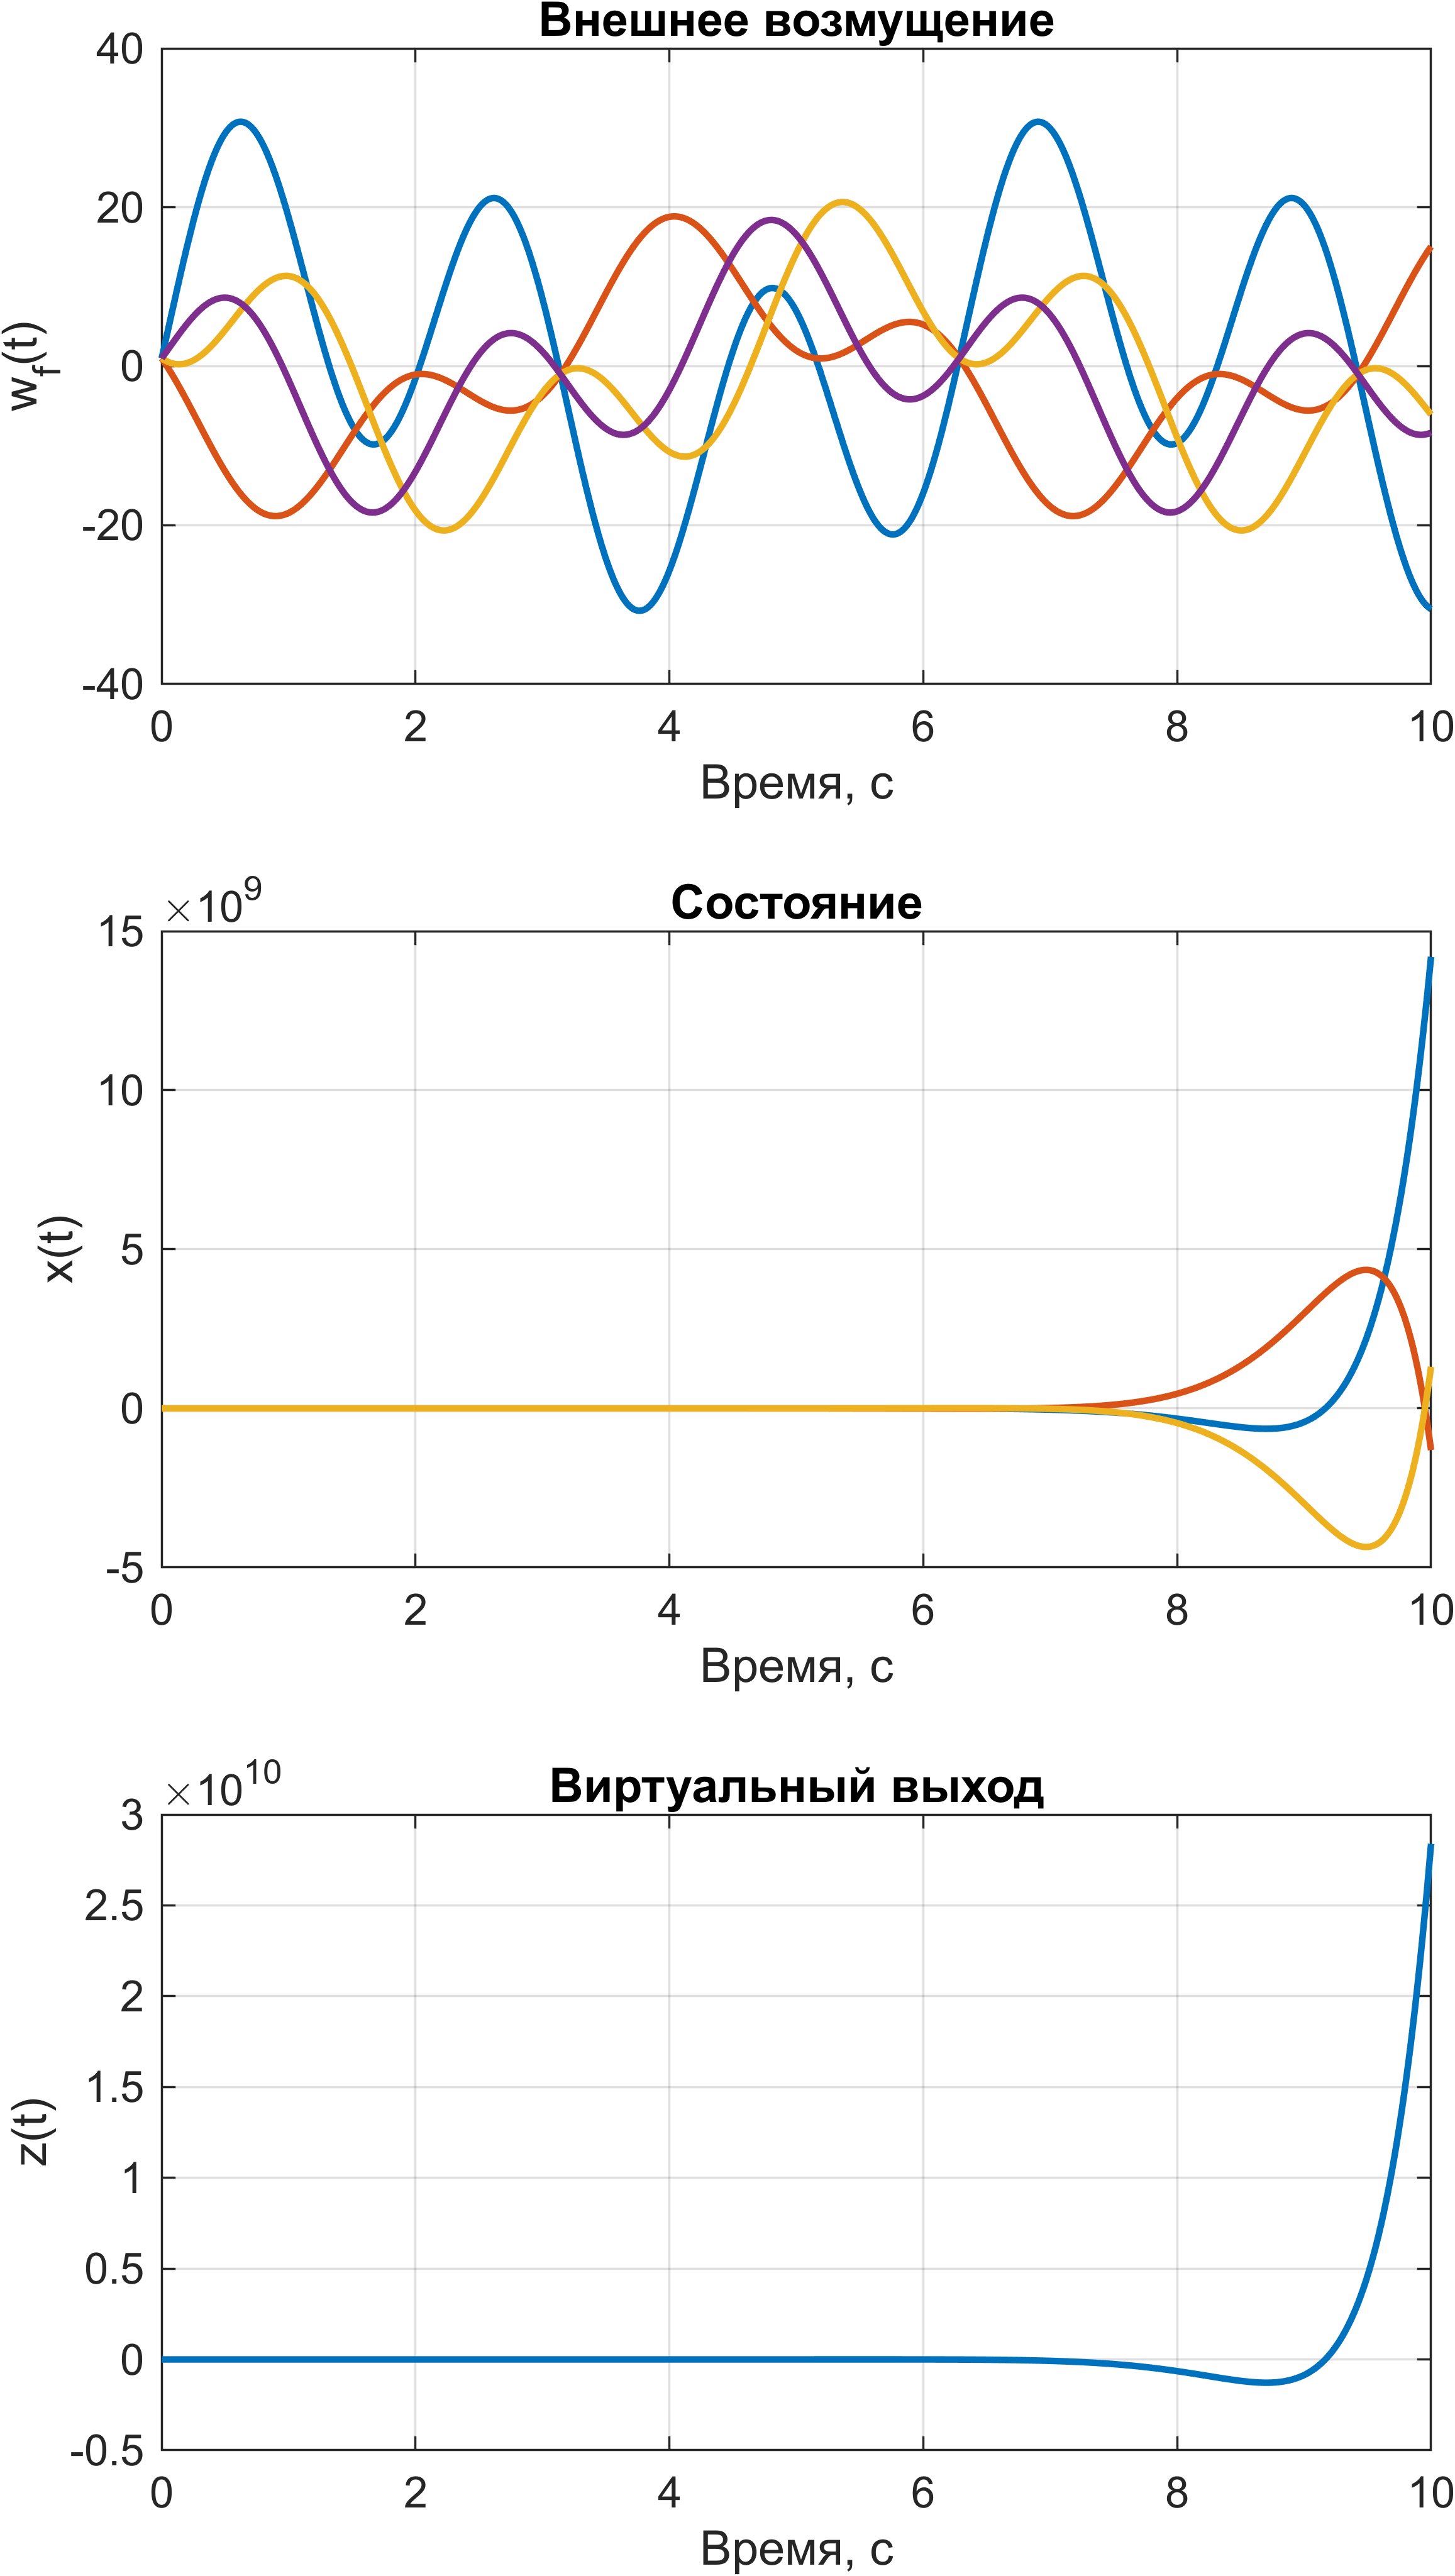
\includegraphics[width=0.8\linewidth]{figs/task1_1.png}
    \caption{Графики разомкнутой системы \eqref{eq:sys1}}
    \label{fig:1.1}
\end{figure}
\begin{figure}[H]
    \centering
    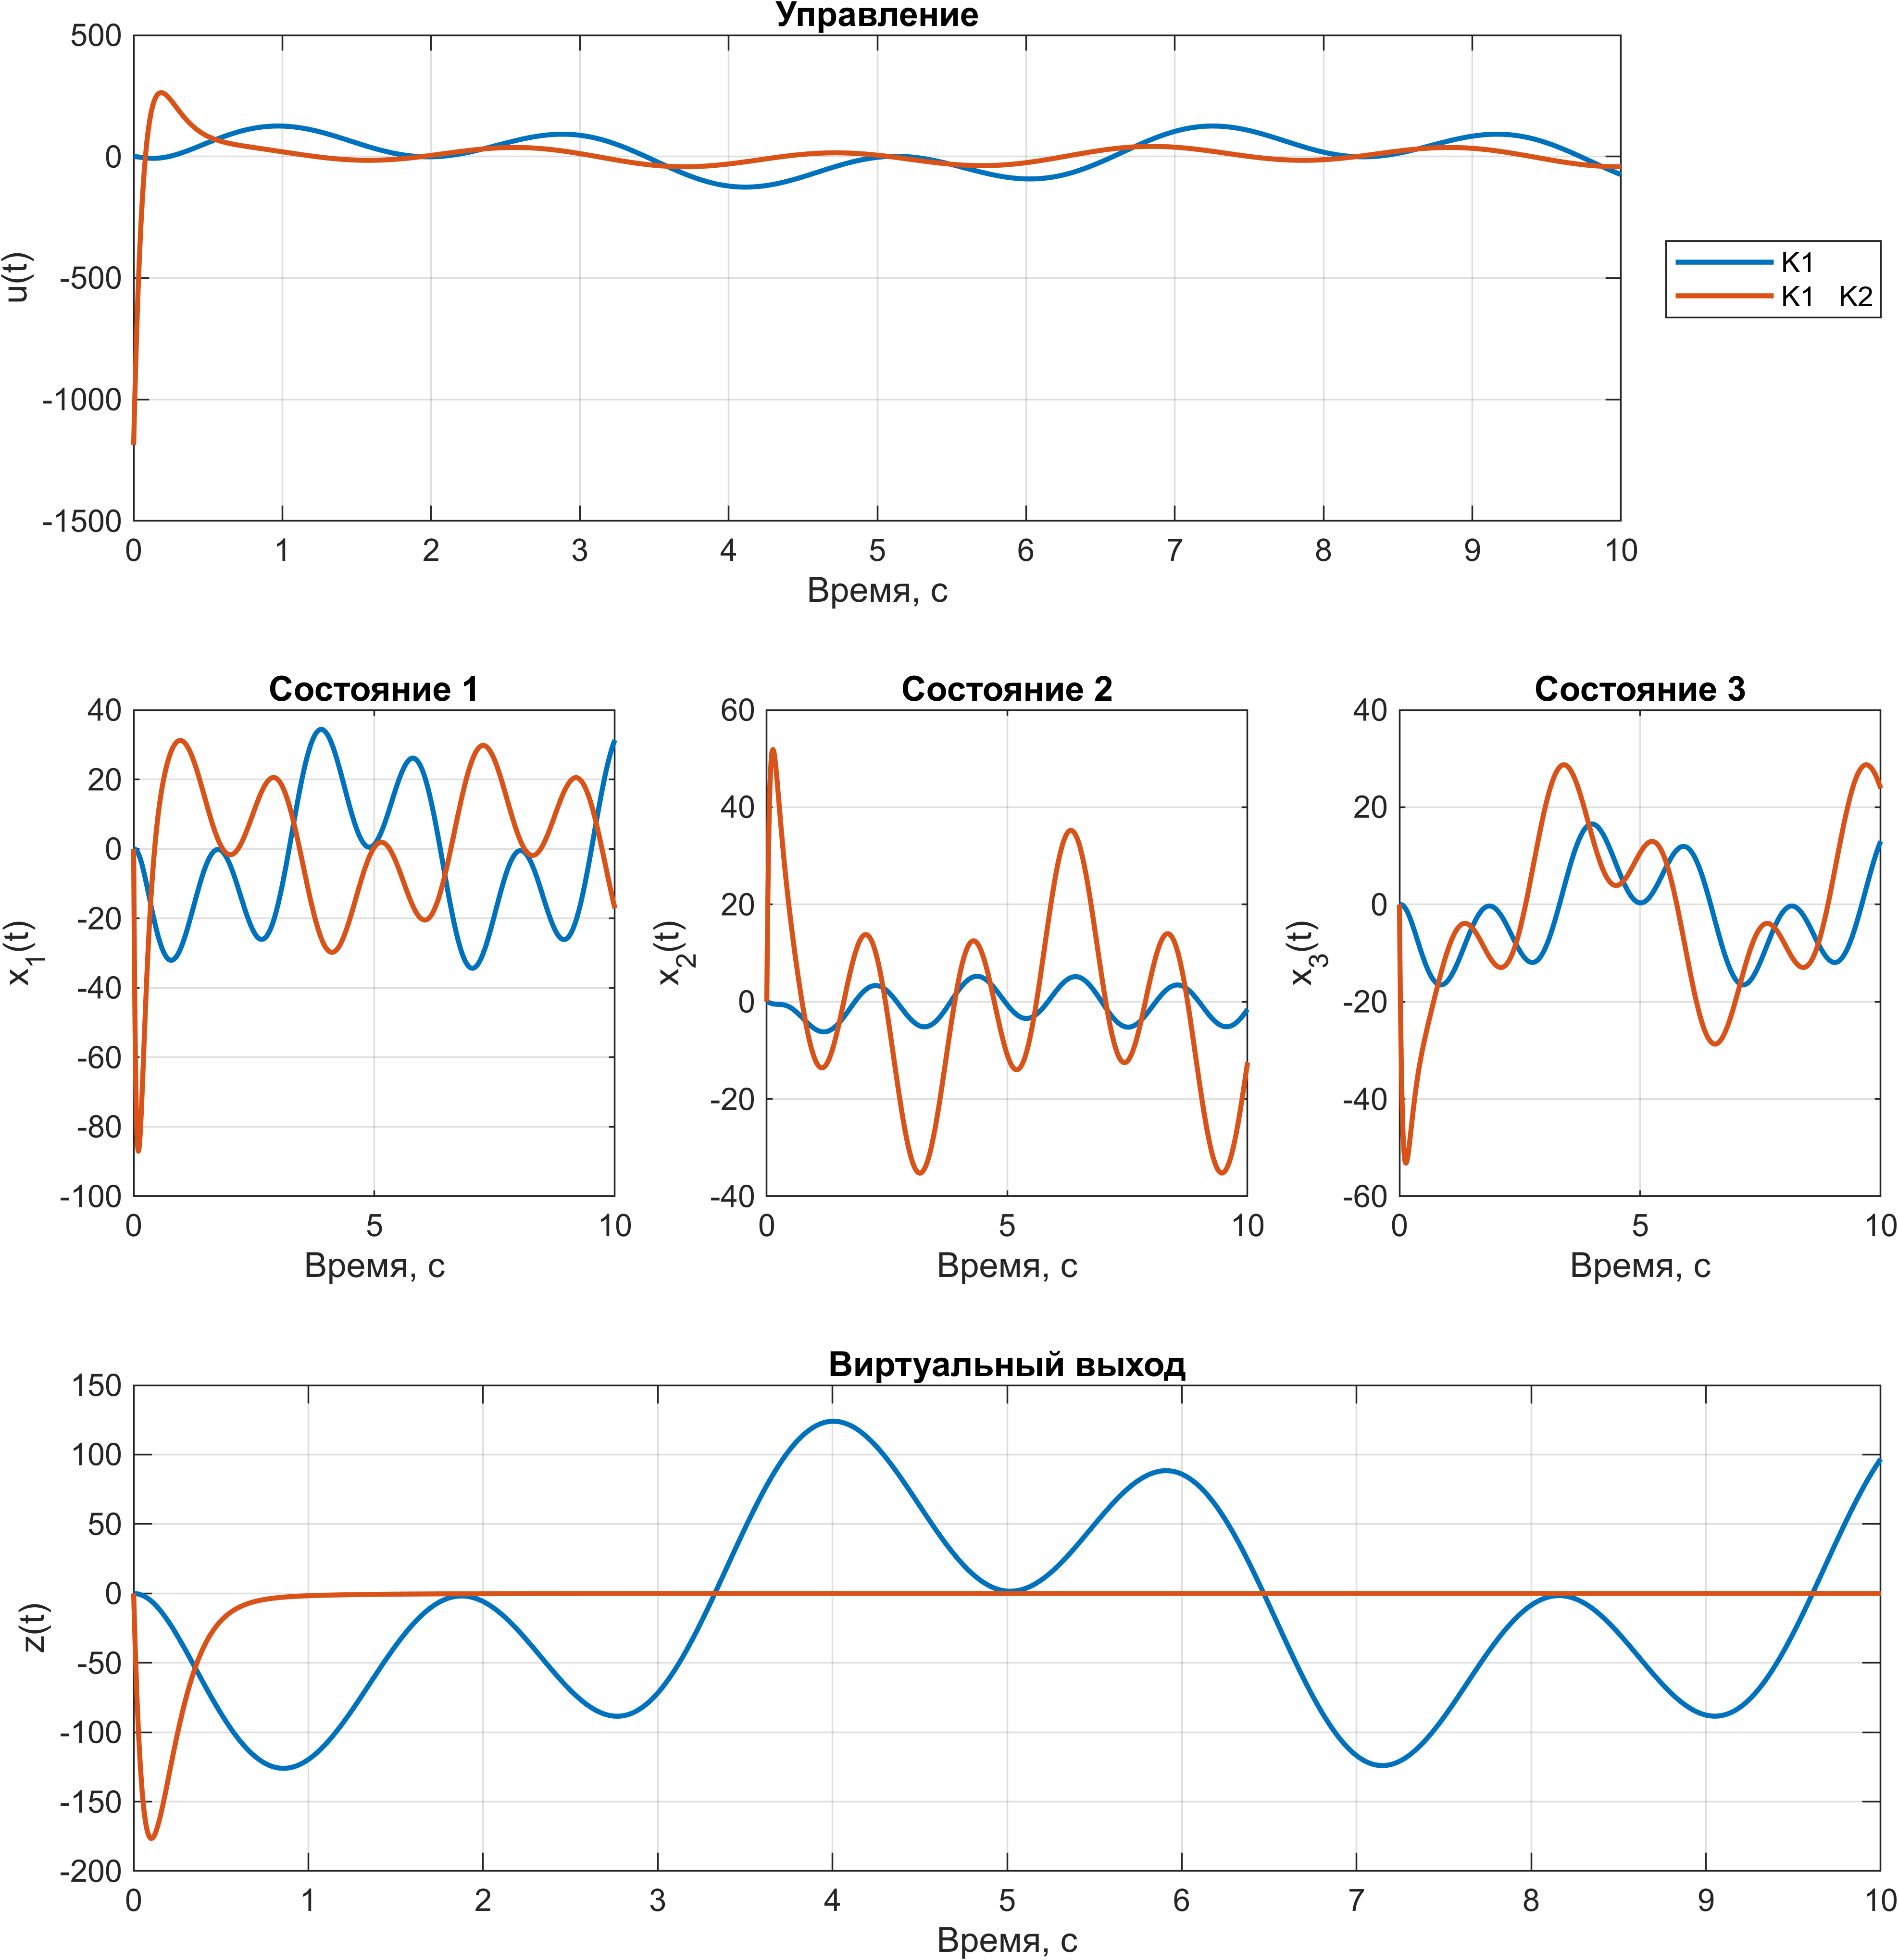
\includegraphics[width=\linewidth]{figs/task1_2.png}
    \caption{Графики замкнутой системы \eqref{eq:sys1} только с ``feedback''-компонентой
    и компенсирующим регулятором \eqref{eq:reg1}}
    \label{fig:1.2}
\end{figure}

\subsection{Вывод}

Был успешно синтезирован компенсирующий регулятор по состоянию, 
состоящий из ``feedback``- и ``feedforward``-компонент. Проведенное 
моделирование показало, что использование только ``feedback``-компоненты 
не позволяет свести виртуальный выход к нулю, тогда как полный 
компенсирующий регулятор эффективно компенсирует внешние возмущения 
и обеспечивает выполнение целевого условия.



\section{Следящий регулятор по состоянию}

\subsection{Анализ системы}
Рассмотрим систему
\begin{equation}
    \dot x=Ax+Bu,\quad x(0)=\begin{bmatrix}
        1&1&1
    \end{bmatrix}^T,
    \label{eq:sys2}
\end{equation}
генератор внешнего возмущения
\begin{equation*}
    \dot w_g=\Gamma w_g,\quad w_g(0)=\begin{bmatrix}
        1&1&1&1
    \end{bmatrix}^T
\end{equation*}
и виртуальный выход вида
\begin{equation*}
    z=C_Zx+D_Zw_g,
\end{equation*}
где
\begin{equation*}
    A=\begin{bmatrix}
        3&5&4\\
        -2&-4&-5\\
        2&2&3
    \end{bmatrix},\quad
    B=\begin{bmatrix}
        2\\-1\\1
    \end{bmatrix},\quad
    C_Z=\begin{bmatrix}
        2&3&3
    \end{bmatrix},
\end{equation*}
\begin{equation*}
    \Gamma=\begin{bmatrix}
        35&56&22&-42\\
        -11&-17&-7&12\\
        -6&-10&-5&10\\
        11&18&6&-13
    \end{bmatrix},\quad
    D_Z=\begin{bmatrix}
        3&4&2&-3
    \end{bmatrix}.
\end{equation*}
Матрица $\Gamma$ абсолютно идентична матрице из \autoref{sec:task1},
поэтому ее спектр и характер возмущения остаются прежними.
Матрицы $A$ и $B$ также не изменились, поэтому система остается
стабилизируемой. Построим схему моделирования системы \eqref{eq:sys2},
замкнутой следящим регулятором
\begin{equation}
    u=K_1x+K_2w_g.
    \label{eq:reg2}
\end{equation}
Ее можно увидеть на \autoref{fig:sys2}.
\begin{figure}[H]
    \centering
    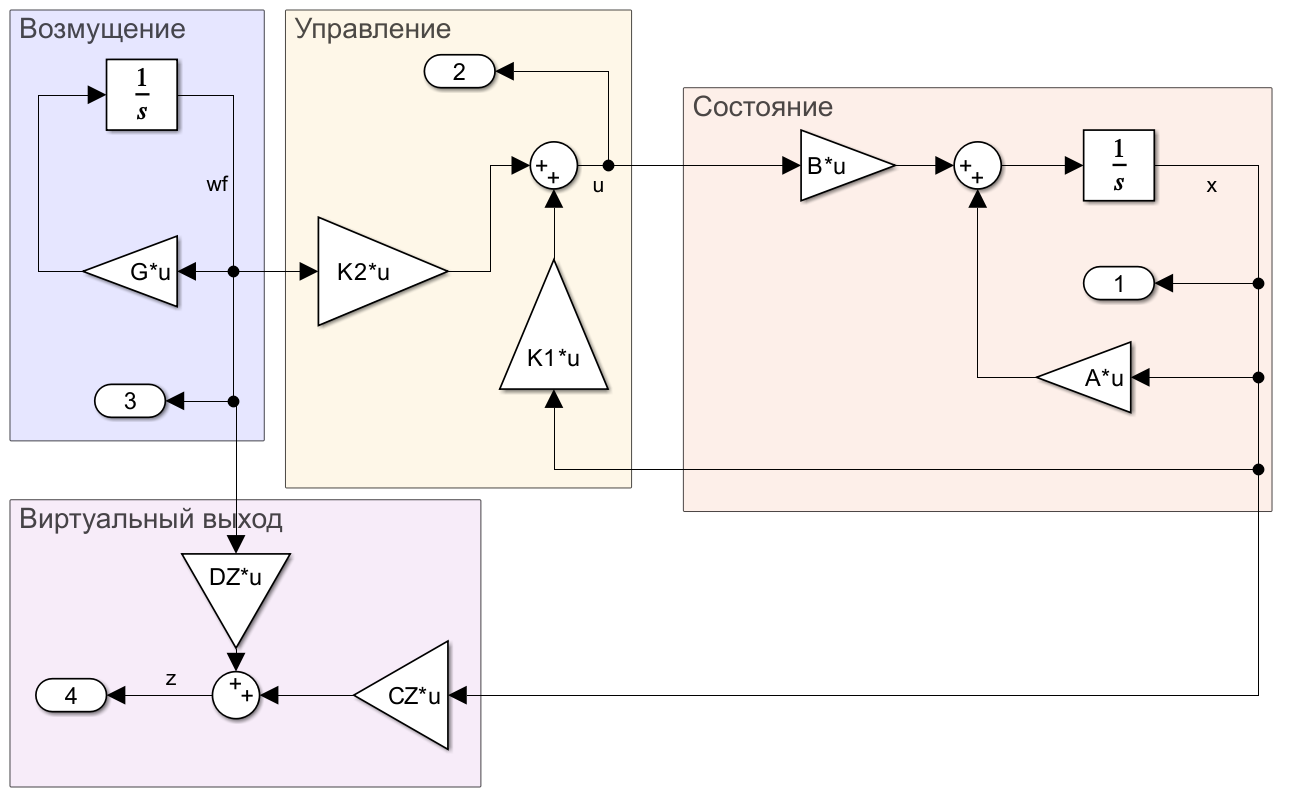
\includegraphics[width=\linewidth]{figs/task2_slx.png}
    \caption{Схема моделирования системы \eqref{eq:sys2}}
    \label{fig:sys2}
\end{figure}
Далее, синтезируем следящий регулятор по состоянию, но
``feedback''-компоненту синтезировать не нужно, возьмем
ее из \autoref{sec:feedback1}, она подойдет, так как
пара ($A$, $B$) не изменилась.

\subsection{Синтез ``feedforward''-компоненты}

Синтезируем «feedforward»-компоненту $K_2$ следящего регулятора \eqref{eq:reg2}.
С помощью CVX решим следующую систему
\begin{equation*}
    \begin{cases}
        P\Gamma-AP=BY\\
        C_ZP+D_Z=0
    \end{cases}
\end{equation*}
относительно $P$ и $Y$ и получим $K_2$
\begin{equation*}
    K_2=Y-K_1P=\begin{bmatrix}
        90.7624&	145.6219&	64.7442&	-109.6806
    \end{bmatrix}.
\end{equation*}

\subsection{Моделирование}
Выполним компьютерное моделирование системы. На \autoref{fig:2.1} графики
разомкнутой системы ($u=0$), по ним видно, что система неустойчива. На
\autoref{fig:2.2} сравнение системы замкнутой только ``feedback''-компонентой
и с компенсирущим регулятором \eqref{eq:reg2}. Использование только $K_1$
компоненты регулятора не смогло свести виртуальный выход к нулю (проследить за 
возмущающим сигналом), но система стала асимптотически устойчивой. 
Компенсирующий же регулятор успешно проследил за возмущением,
сведя виртуальный выход к нулю.
\begin{figure}[H]
    \centering
    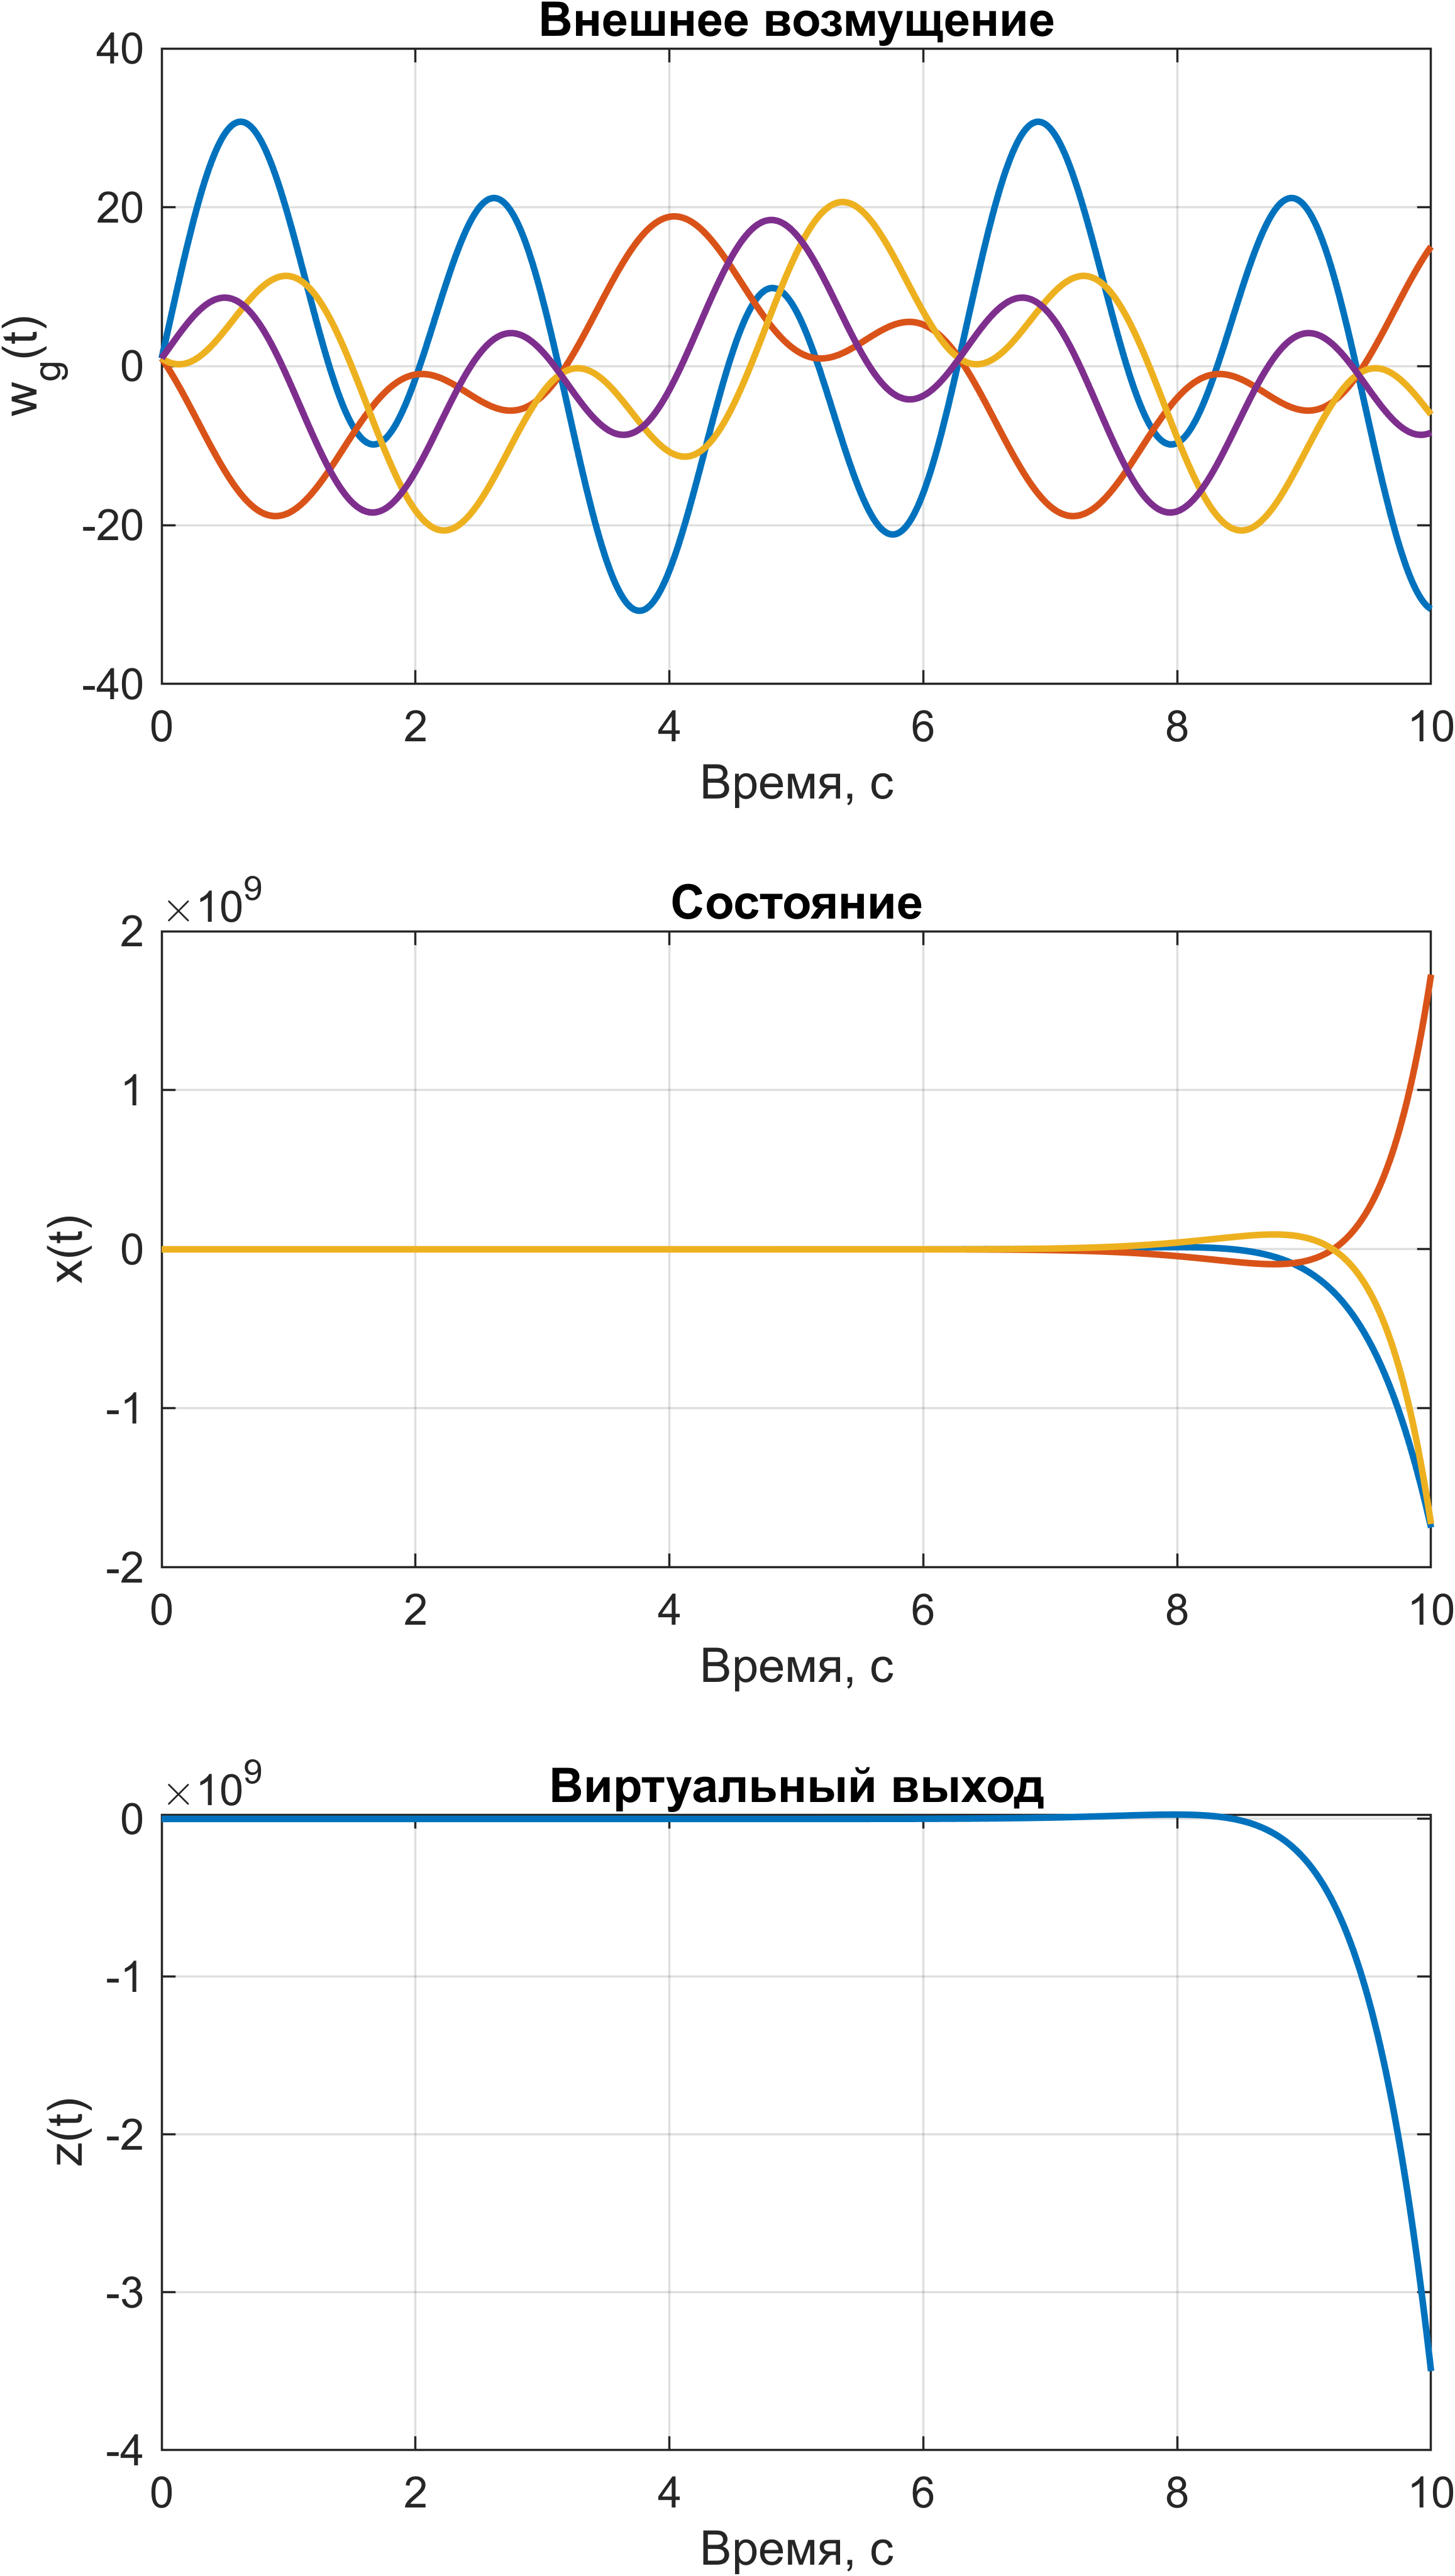
\includegraphics[width=0.8\linewidth]{figs/task2_1.png}
    \caption{Графики разомкнутой системы \eqref{eq:sys2}}
    \label{fig:2.1}
\end{figure}
\begin{figure}[H]
    \centering
    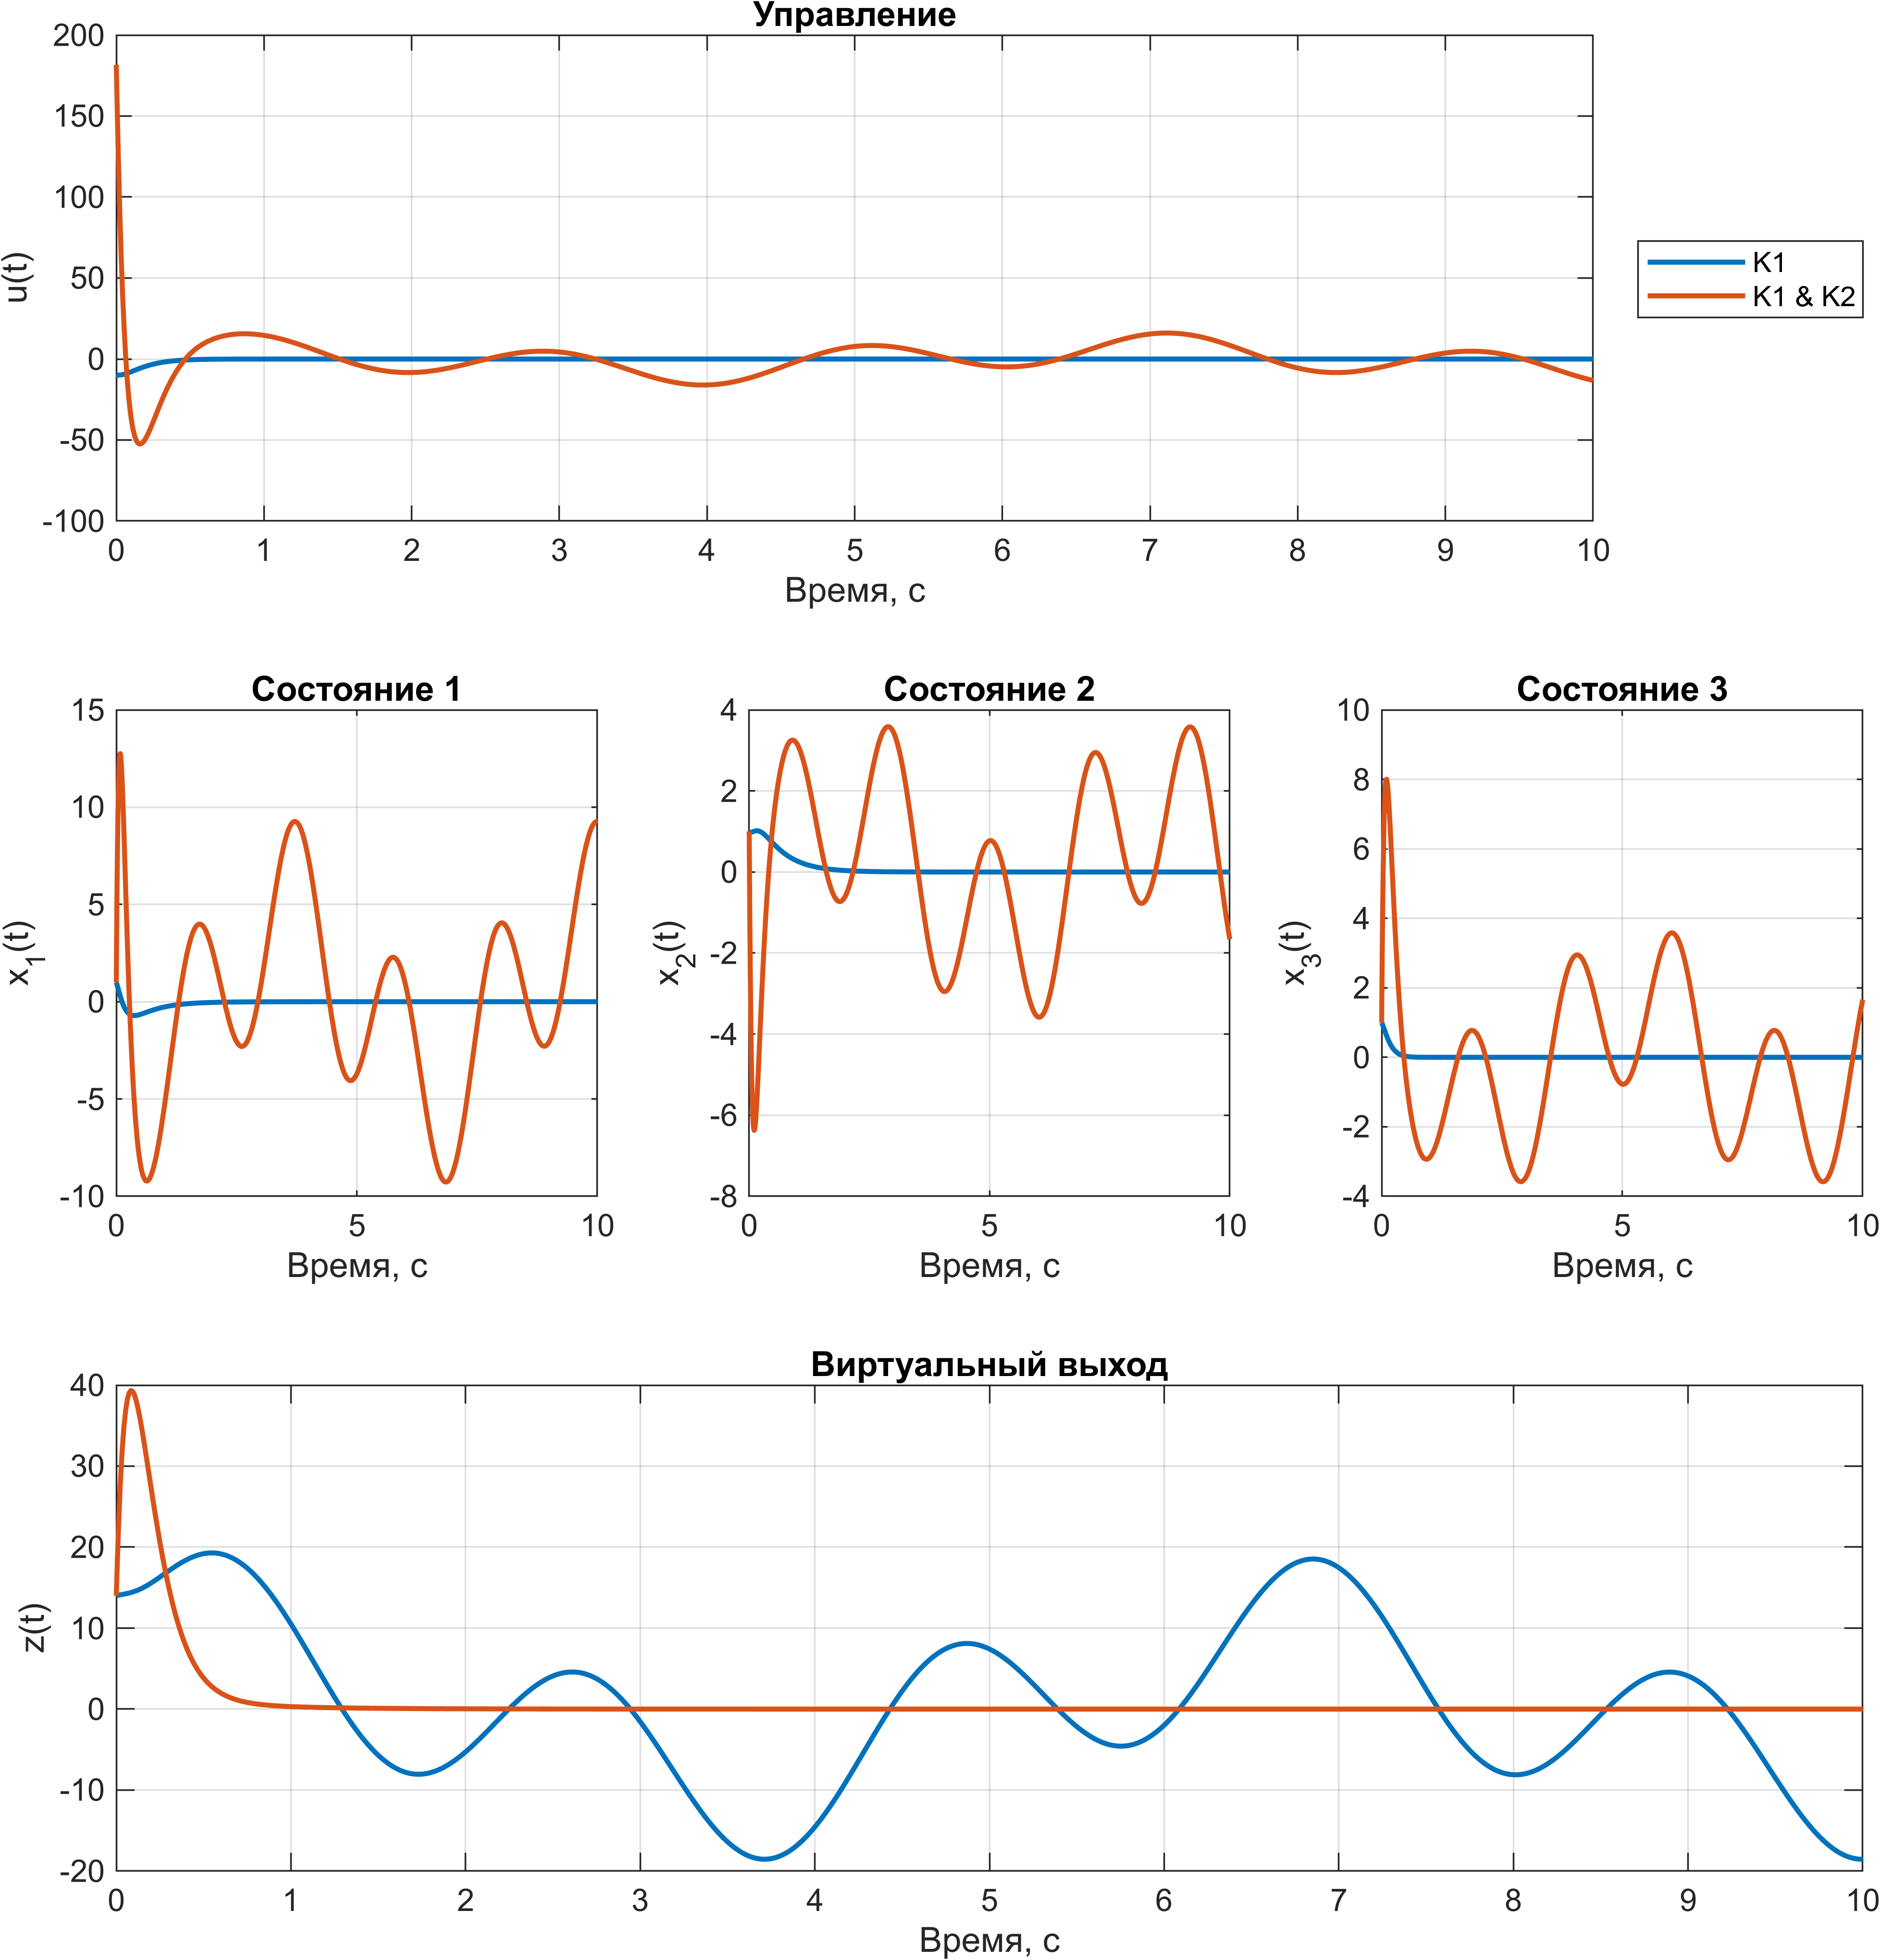
\includegraphics[width=\linewidth]{figs/task2_2.png}
    \caption{Графики замкнутой системы \eqref{eq:sys2} только с ``feedback''-компонентой
    и с компенсирующим регулятором \eqref{eq:reg2}}
    \label{fig:2.2}
\end{figure}

\subsection{Вывод}

Был успешно синтезирован следящий регулятор по состоянию, состоящий 
из ``feedback``- и ``feedforward``-компонент. Проведенное моделирование 
показало, что использование только ``feedback``-компоненты делает 
систему асимптотически устойчивой, но не позволяет свести виртуальный 
выход к нулю. Полный следящий регулятор успешно следит за внешним
возмущением и обеспечивает выполнение целевого условия.


\newpage
\section{Слежение и компенсация по выходу}

